\section{\texorpdfstring{Hash functions, Merkle trees, MACs}{Hash functions, Merkle trees, MACs}}
\vspace{5mm}
\large

\begin{definition}
	Hash function $f$ is
	\[ f:\{0, 1\}^{\ast} \to \{ 0,1 \}^b \]

	Typically used for signatures.
\end{definition}

\begin{properties} Secure hash function:
	\begin{enumerate}
		\item collision-free: there are no $x \neq y: h(x) = h(y)$
		\item no second preimage: for given $x$, find $y$: $h(x) = h(y)$.
		\item no inversion: for given $z$ find $x: h(x) = z$.
	\end{enumerate}

\end{properties}

\subsection{Merkle-Damgard construction}
Given a \emph{compression function} $f:\{0, 1 \}^b \times \{0, 1 \}^b \to \{0, 1 \}^b$. Construct $h$:

	\includegraphics[scale=0.4]{md.eps}

\begin{theorem}[Collision resistant hash]
	If $f$ is collision resistant compression function $\Rightarrow h$ is collision resistant hash function.
\end{theorem}
\begin{proof}
	Indirect proof. Assume we found a collision of $h$, meaning $h(x_1,...,x_n) = h(x_1^{\prime},...,x_n^{\prime})$

	Let's consider 2 options:\\
	1) $n \neq n^{\prime}$. In the last step we compress $n$ and $n^{\prime}$. As outputs are identical $\Rightarrow$ the last block containing size is also identical. Therefore we have found collision of $f$.\\
	2) $n = n^{\prime}$. Using induction we examine compressed blocks. As outputs are identical: either the blocks were identical or we have found collision of $f$. Then, as messages are not identical, there exist two different blocks encoded to the same output. Which implies collision of $f$.
\end{proof}

\subsubsection{Length extension property of M-D hash} Suppose we have a message $x$ and prefix $p$.
For a Random function, knowing prefix $h(p)$ should help us producing full $h(p | s)$. Where $s = x - p$ suffix.

From the M-D internal structure, hash of the suffix depends on the hash of prefix.
Therefore, an attacker, knowing hash of the prefix, can add his data to the message and compute new signature (hash).

We should take this property into consideration using M-D hashes.

\subsubsection{Compression function for M-D}

Having a block cipher, we can use it to create compression function as the following:
\[ f(u,v) := E_u(v) \oplus v \]

XOR is required because otherwise finding collision is easy. Suppose $f(u,v) := E_u(v)$, then
\[ E_u(v) = y \]
Taking another key, e.g. $b$, we decrypt $y$ using $b$
\[ D_b(y) = a \Rightarrow f(u,v) = y = f(a,b) \]

Using DES as block cipher is also a bad idea, since $E_{\overline{k}}(\overline{x}) = \overline{E_k(x)}$:
\[ f(\overline{a}, \overline{c}) = E_{\overline{a}}(\overline{c}) = \overline{E_a(c)} \oplus \overline{c} = E_a(c) \oplus c = f(a,c) \]

For $v := D_u(0), f(u,v) = E_u(v) \oplus v = 0 \oplus v = v$. Which cannot happen for random hash function.

\begin{theorem}[Collision resistant hash]
	With an ideal block cipher (for every key a random permutation) $f$ is collision resistant. In particular, for an attack evaluating E/D $q$ times ($q \leq 2^{b/2}$)
	\[ Pr[collision] \leq q^2/2^b \]
\end{theorem}
\begin{proof}
	WLOG: attacker do not ask redundant questions (E of the text he already knows).

	From the properties of ideal block cipher, results of encryption is a bijection. Can be viewed as table of values.

	Asking E and D questions attacker gets following answer:
	\[ E_u(v) = f(u,v) = E_u(v) \oplus v \land D_u(v) = f(u, D_u(v)) = v \oplus D_u(v) \]

	We find first collision in step $i: 1 \geq i \leq q$. We found $f(l,k)$ matching some known value, having $(i - 1)$ of them.
	So it was either the answer to E or D question, which is exactly 1 value.

	For every pair, known and new answers:
	\[ Pr[collision] = \frac{1}{num\ of\ possible\ ans.} \leq \frac{1}{2^b - i - 1} \land i \leq 2^{i/2} \leq 2^{b/2} \Rightarrow Pr[collision] \leq \frac{1}{2^{b-1}} \]

	\[ Pr[collision] \leq \frac{1}{2^{b-1}} pairs \leq \frac{1}{2^{b-1}} \binom{q}{2} \leq \frac{q^2}{2*2^{b-1}} = \frac{q^2}{2^{b}} \]

\end{proof}

\subsubsection{Finding collision of hash function}

\begin{enumerate}
	\item Brute force: by the Birthday paradox expect a match in $\approx 2^{b/2}$ steps. Lots of memory.
	\item With constant memory. Assume $\forall x: |x| = |h(x)|$.
		Let's construct a graph where vertexes are all possible blocks and edges are $(x, h(x))$.
		Degree of every $x$ is 1. Iterating $h(h(... h(x))$ we create a path in Graph.
		At some point there will be a loop, as Grah is finite.

		A subgraph reachable from $x$ looks like lollipop. Path + cycle.
		In order to find collision in such subgraph we choose 2 travelers in the graph: tortoise (1 step at time) and rabbit (2 steps at time).
		Starting at $x$, they move in graph. Claim: they will meet in vertex which connects path with cycle.
	\item In many cases we need to find meaningful collision (to send evil message instead of innocent).
		And the party signing messages refuses to sign random noise.

		In order to find collision, we construct parametrized message. Let's say Dear Bob, Dear Sean etc.
		With $k$ places of parametrization we can produce $2^k$ innocent messages.

		Both previous attacks work with such messages. However, edges in the Graph for 2nd type of attach will be $(x, h(parametrize(x)))$.
	\item Meet-in-the-middle attack. We want $h(evil) = h(innocent)$.

		Let A,B two random subsets of all hashes. Than, with high probability they have non empty intersection. $|A| = |B| = \sqrt{n}$.
		A will be hashes of $2^{b/2}$ innocent messages, B - hashes of $2^{b/2}$ evil messages.
	\item For M-D hashes we can product lots of collision, as easy as 1.
		By Birthday paradox, we find first collision: $x_1 \neq x_1^{\prime}: f(IV, x_1) = f(IV, x_1^{\prime}) = y_1$.
		Then we repeat $k$ times using $y_{i-1}$ as IV. As we can use both $x_i$ and $x_i^{\prime}$ to get $y_{i-1}$.
		We get $2^k$ combinations which hash to the same result.

		As a result, concat of 2 hashes, both with length $b$ does not have security level $2b$ if either of functions is M-D.
		Because we can find $2^{b/2}$ colliding messages in time $b/2 * 2^{b/2}$. Than $h_2$ is likely to have 2 collisions.
		Therefore, we have found collision in $h = h_1 | h_2$ in time $b/2 * 2^{b/2}$.
\end{enumerate}

\subsection{Sponge construction}
Sponge construction has 2 phases:\\
1) Absorbing the input (updating internal state depending on input)\\
2) Squeezing the output

\begin{example}
	SHA-3 sponge construction. Suppose we have a permutation $\pi$ on blocks of size $w = r + c$.
	Where $w$ is width, $r$ - rate and $c$ - capacity.

	\includegraphics[scale=0.3]{sponge.eps}

	Security against BF attacks:\\
	1) By the Birthday paradox we can attack the output in $2^r$ steps.\\
	2) Internal collisions (chosen plain text attack):\\
	By the Birthday paradox in $2^c$ steps we can find
	\[ i < j: S_i = S_j \]
	In order to get collision, we feed the sponge $0^i$ as first part of input.
	Then we feed $(t_i \oplus t_j)$ to get $r = t_i$ back and feed zeros till the end $0^{j - 1}$.
	As a result, after $j$-th stage sponge squeezes the same output.

	However, we know that for a random $\pi$ security level $\geq \min(r/2, c/2)$.
\end{example}

\subsection{Other hash functions}

\textbf{Shake-128}, an XOR(extensible-output functions)
Designed for variable size output. Can be used as PRNG, that is initialized by some value.
Can be run for many \# of steps.

\begin{definition}
	Merkle trees. Divide data into blocks, then hash and concat some of then.
	Which forms a tree.

	\includegraphics[scale=0.3]{merkle.eps}

	Claim: if hash function $f$ is collision-free $\Rightarrow$ whole tree is collision-free.

	Can be run in parallel, also updating a single block of data result in path update only.
	Used in practice to sign a DB state.
\end{definition}

\begin{observation}
	Naive Merkle tree is not secure to \emph{extension attacks}.
	As we can take old tree, add another subtree(that includes our evil data) and a new root.

	Fix: add 1 bit to every node, 1 is for Root. (see Sakura coding as example).
\end{observation}

\subsection{MACs}
MACs are used to sign some information (either plain or cipher text).

\includegraphics[scale=0.3]{mac_0.eps}

Usually, sign is deterministic and verification is just sign + compare with received signature from the counterparty.
Typically sign is parametrized hash.

\paragraph{Security Model}
Attacker has access to \emph{signing oracle} and can ask it to sign $(x_1, ..., x_n)$ plain texts.
Cryptographic primitive is secure iff the attacker is able to produce new valid signature for $x \neq x_i$.

How to sign? One can include a key to the hash alongside the text. There are several ways to do so:

\begin{itemize}
	\item $h(k | x)$ is secure for random $h$, but not for Merkle-Damgard.
		M-D hashes are not protected against extension attacks. SHA-3 is believed to be secure for such usage. Such construction is included to the standard as \textbf{KMAC}.
	\item $h(x | k)$ will not work either, because the attacker can precompute all combinations independent from key, then try with specific key. Therefore, $h(x | k)$ should be also avoided.
	\item Much better option is \textbf{HMAC}$_h := h(k \oplus C_{out} | h((k \oplus C_{in}) | x))$.
	$C_{in}, C_{out}$ are derived from master key. Where $h((k \oplus C_{in}) | x)$ is collision-resistant. Consequently, we can even use broken SHA-1,2.
\end{itemize}

\paragraph{Combining auth with enc}
Typically, we want both security and authenticity, so that the attacker cannot neither decrypt nor change the message. To achieve that, MAC with encryption is used.
Again, there are several possibilities to combine 2 primitives.

\begin{itemize}
	\item Encrypt and MAC independently is a bad idea, since the signature of the same message encrypted with different cipher is leaking their identity.
	\item MAC then Encrypt has several advantages over the opposite option:\\
		1) Signature should reflect plain text as close as possible. Should be same for different ciphers.\\
		2) Authenticity is more important than secrecy (e.g. for nuclear missiles control system)\\
		3) MAC is protected by the cipher

		Unfortunately, described scheme is vulnerable to the \emph{oracle timing attack}.
		Specifically, reducing the padding by 1 block will result in 1 MAC iteration less.
		Which can be observed by the attacker. As a result, almost all protocols that includes MAC then Encrypt are broken because of this attack.

		However, MAC then Encrypt is used in TLS, To avoid the attack, chosen MAC is not the block type.
	\item Encrypt then MAC is the recommended scheme.
\end{itemize}

\paragraph{CBC-MAC}
We can construct MAC from symmetric cipher in CBC mode.

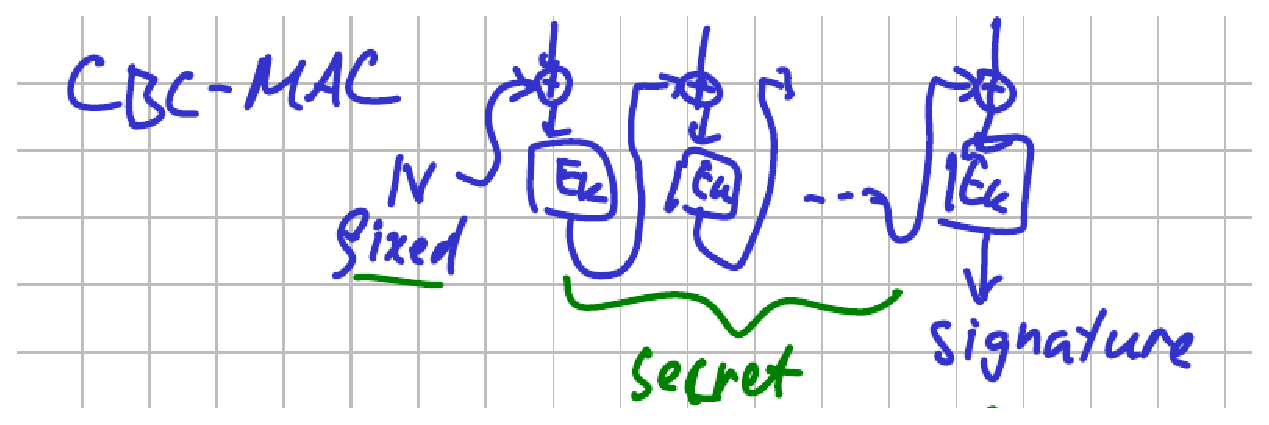
\includegraphics[scale=0.4]{mac_1.eps}

\begin{properties}
In order to be secure, CBC-MAC should have these properties

\begin{itemize}
	\item Fixed IV. If the IV is random (not fixed), it should be transfered over the network.
		As a result, Mallory can flip bits in both IV and the first block of the message.
		Which will alter the message, but the sign remains valid.
	\item Intermediate steps of the CBC should be kept secret.
	\item No message is a prefix of another message.
\end{itemize}
With these properties, assuming ideal cipher, CBC-MAC is proved to be secure.
\end{properties}

\begin{definition}
	An MAC is \emph{Shannon secure} iff given a known pair $(x, sign(x))$ all signatures of $x^{\prime} \neq x$ are equally possible for a random key.
	Where $sign(x)$ is a signing function which uses a single random key.

	Alternatively, a pair $(x, sign(x))$ gives no info about other messages.
\end{definition}

\begin{definition}
	A family of functions from set X to set Y is $\mathcal{H} := \{ h_k | k \in \mathcal{K} \}$.
	Technically a multiset.
\end{definition}

\subsubsection{2 independent MAC}

\begin{definition}
	$\mathcal{H}$ is 2-independent iff
	\[ \forall x, x^{\prime} \in X \forall y, y^{\prime} \in Y: Pr_h[h(x) = y \land h(x^{\prime}) = y^{\prime}] = \frac{1}{|Y|^2} \]
\end{definition}

Typically we use Galois field (GF) as X and Y.

\begin{example}
	$h_{a,b}(x) := ax + b$ is a 2-independent family of functions. To construct a MAC from this family we:\\
	1) select $h \in \mathcal{H}$ at random \\
	2) key is $(a,b)$ - parameters of $h$\\
	3) signature is $h(x)$.

	To prove 2-independence we calculate ($x_1, x_2, y_1, y_2$ are given constants):
	\[ Pr_f[ h_k(x_1) = y_1 \land h_k(x_2) = y_2] = Pr_{a,b}[ax_1 + b = y_1 \land ax_2 + b = y_2] \]
	As we have system of 2 linear equations with 2 unknowns: a and b, it has an unique solution.
	Therefore the probability is $\frac{1}{|Y|^2}$, all possible choices of parameters a, b.
\end{example}

\begin{theorem}[2-ind MAC security]
	2-ind MAC is Shannon secure.
\end{theorem}
\begin{proof}
	By the conditional probability:
	\[ Pr_f[ h_k(x_1) = y_1 | h_k(x_2) = y_2] = \frac{Pr_f[ h_k(x_1) = y_1 \land h_k(x_2) = y_2]}{Pr_f[h(x_1) = y_1]} \]
	By the 2-independence
	\[ Pr_f[ h_k(x_1) = y_1 \land h_k(x_2) = y_2] = \frac{1}{|Y|^2} \]
	%TODO do not understand why (lecture 11.25, from 1:14:00)
	$Pr_f[h(x_1) = y_1]$ can be calculated as a disjoint sum of events
	\[ \sum_{y_i} Pr_h[h(x) = y \land h(x_i) = y_i] = \frac{|Y|}{|Y|^2} \]
	Combining 2 results
	\[ Pr_f[ h_k(x_1) = y_1 | h_k(x_2) = y_2] = \frac{1}{|Y|^2} \div \frac{1}{|Y|} = \frac{1}{|Y|} \]
	Which satisfies Shannon security.
\end{proof}

Downsides of 2-ind MAC:
\begin{itemize}
	\item key is twice as large as a message.
	\item no key can be reused
	\item sequence number is required
	\item message size = signature size
\end{itemize}

\subsubsection{Polynomial based MAC}
Suppose, F is Galois field, $X = F^n, Y = F, K = F^2$. Then
\[ h_{a,b}(x_1,...,x_n) = x_1a^n + ... + x_na + b \]
Evaluation the polynomial at some point could be done in $\bigO(n)$.

\begin{theorem}[Polynomial MAC security]
	Polynomial MAC is not Shannon secure.
\end{theorem}
\begin{proof}
\[ Pr_{a,b} [h_{a,b}(x_1^{\prime},...,x_n^{\prime}) = y^{\prime} | h_{a,b}(x_1,...,x_n) = y] = Pr_{a,b}[L | R] = \frac{Pr[L \land R]}{Pr[R]} \]
Substracting 1st equation from second we get
\[ Pr[L \land R] = (x_1 - x_1^{\prime})a^n + ... + (x_n - x_n^{\prime})a = y - y^{\prime} \]
Which is a non zero polynomial, since messages are different $\Rightarrow$ at most $n$ values of a.
Also, initial equation was satisfied for exactly one $b \Rightarrow$ at most $n$ pair $(a, b)$. Yielding:
\[ Pr[L \land R] \leq \frac{n}{|F|^2} \]
Then
\[ Pr[R] = \frac{|F|}{|F|^2} = \frac{1}{|F|} \]
And
\[ Pr_{a,b}[L | R] \leq \frac{n}{|F|} \]
Which does not satisfy Shannon security, as $n$ is in numerator. However, we can choose reasonably big Field.

\end{proof}

And yet, polynomial MAC is not practical as we need a new random key for every message.
Which can be solved by using PRNG parametrized by key.
\begin{observation}
	If parameter $a$ is fixed and $b$ is generated by PRNG security level does not decrease.
\end{observation}

\subsubsection{GCM mode of block ciphers}

\begin{definition}
	GCM (Galois counter mode) is an auth encoding with additional data (e.g. sign, sequence number)

	\includegraphics[scale=0.4]{gcm.eps}

	We use additional data, encoded data, sizes and IV as a coef of a Polynomial. And $P(E_k(0))$ is a signature, where $E_k(0)$ is a constant than has to be secret!

	As elements are 128-bit strings, addition is XOR multiplication of polynomials over field $\Z_2$.
	Which is a \emph{carry-less} multiplication mod some irreducible polynom Q.
\end{definition}

\begin{example}
	Poly 1305 [Bernstein], is a MAC construction from block ciphers over $GF(2^{130} - 5)$.
	Size of the field is choosen close to power of 2 for speedup. Moreover, points $a$ in which polynomial is evaluated are also some specific subset of the field for the same reason.
	Security level does not decrease significantly.
\end{example}

